% -*- compile-command: "make HOCKING-chip-seq-slides.pdf" -*-
\documentclass{beamer}
\usepackage{tikz}
\usepackage[all]{xy}
\usepackage{amsmath,amssymb}
\usepackage{hyperref}
\usepackage{graphicx}
\usepackage{algorithmic}

\DeclareMathOperator*{\argmin}{arg\,min}
\DeclareMathOperator*{\Lik}{Lik}
\DeclareMathOperator*{\Peaks}{Peaks}
\DeclareMathOperator*{\Segments}{Segments}
\DeclareMathOperator*{\argmax}{arg\,max}
\DeclareMathOperator*{\maximize}{maximize}
\DeclareMathOperator*{\minimize}{minimize}
\newcommand{\sign}{\operatorname{sign}}
\newcommand{\RR}{\mathbb R}
\newcommand{\ZZ}{\mathbb Z}
\newcommand{\NN}{\mathbb N}

\begin{document}

\title{Statistical machine 
learning algorithms for 
understanding big data in
  genomics and medicine}

\author{
  Toby Dylan Hocking\\
  toby.hocking@mail.mcgill.ca
}

\maketitle

\begin{frame}
  \frametitle{Supervised learning example: image classification}
  \begin{tabular}{cc}
  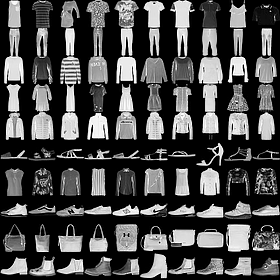
\includegraphics[width=2in]{fashion-mnist-sprite-some}  &
  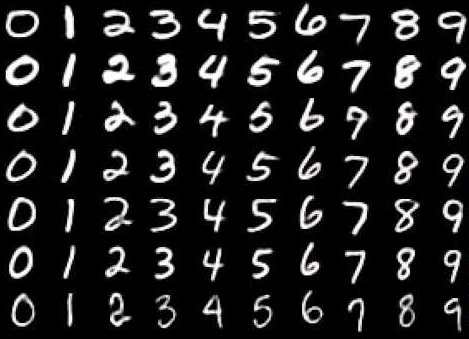
\includegraphics[width=2in]{mnist-digits}
  \end{tabular}
  


  Sources: github.com/zalandoresearch/fashion-mnist, github.com/cazala/mnist
\end{frame}

\begin{frame}
  \frametitle{Labeling enables supervised machine learning algorithms}
  \begin{tabular}{ccc}
    Photos & Cell images & Copy number profiles \\
    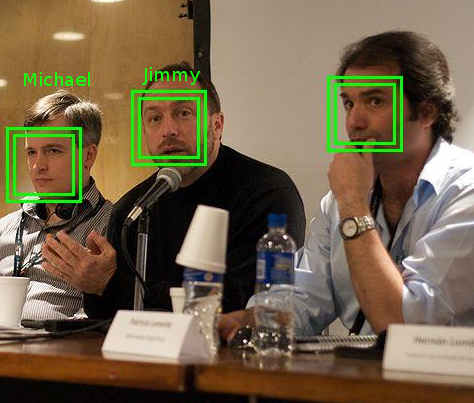
\includegraphics[width=1.3in]{faces} &
    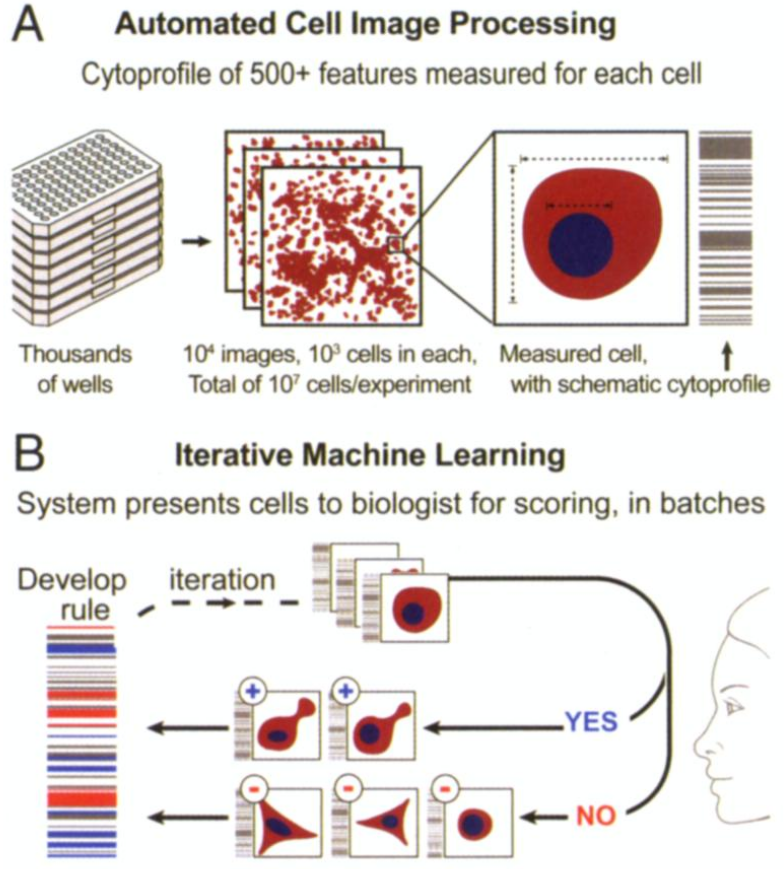
\includegraphics[width=1.3in]{cellprofiler} &
    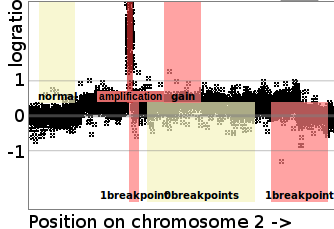
\includegraphics[width=1.5in]{regions-axes}\\
    Labels: names & phenotypes & alterations \\ \\
    CVPR 2013 & CellProfiler & SegAnnDB \\
    246 papers & 873 citations & Hocking et al, 2014. \\
     &
  \end{tabular}
  Sources: \url{http://en.wikipedia.org/wiki/Face_detection}\\
  Jones et al PNAS 2009. Scoring diverse cellular morphologies in
  image-based screens with iterative feedback and machine learning.
\end{frame}

\begin{frame}
  \frametitle{DNA COPY NUMBER ANALYSIS}
\end{frame}

\begin{frame}
  \frametitle{SegAnnDB demo}
    A good example of false negatives to correct on chr1 and chrX
  \url{http://bioviz.rocq.inria.fr/profile/GSM313887/}
\end{frame}

\begin{frame}
  \frametitle{copy from here}
  http://members.cbio.mines-paristech.fr/~thocking/papers/2012-10-12-Learning-penalties-for-change-point-detection/penalty-learning-slides.tgz
\end{frame}

\begin{frame}
  \frametitle{PEAK DETECTION IN CHIP SEQ DATA}
  
\end{frame}

\begin{frame}
  \frametitle{Chromatin immunoprecipitation sequencing (ChIP-seq)}
  Analysis of DNA-protein interactions.

  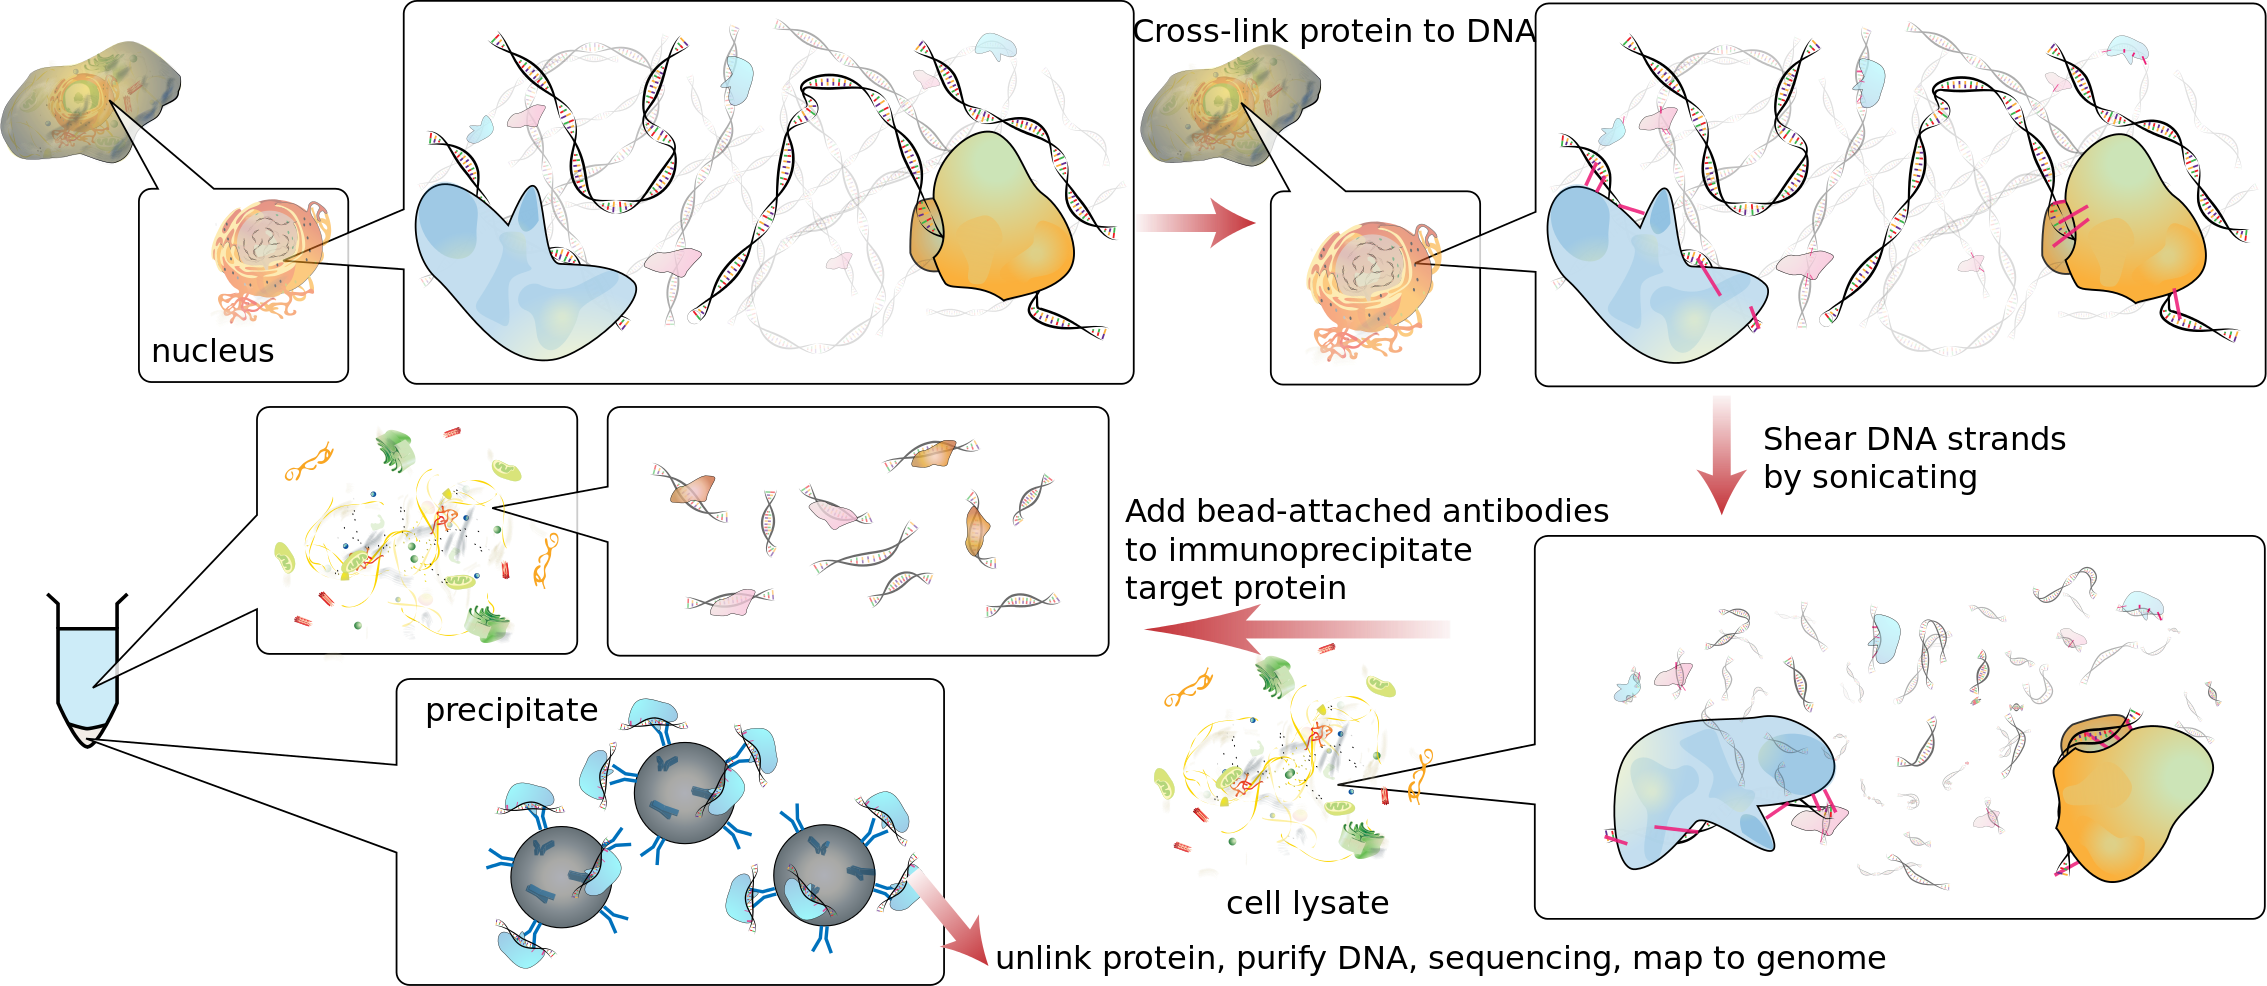
\includegraphics[width=\textwidth]{Chromatin_immunoprecipitation_sequencing_wide.png}

  Source: ``ChIP-sequencing,'' Wikipedia.
\end{frame}

\begin{frame}
  \frametitle{Problem: find peaks in each of several samples}
  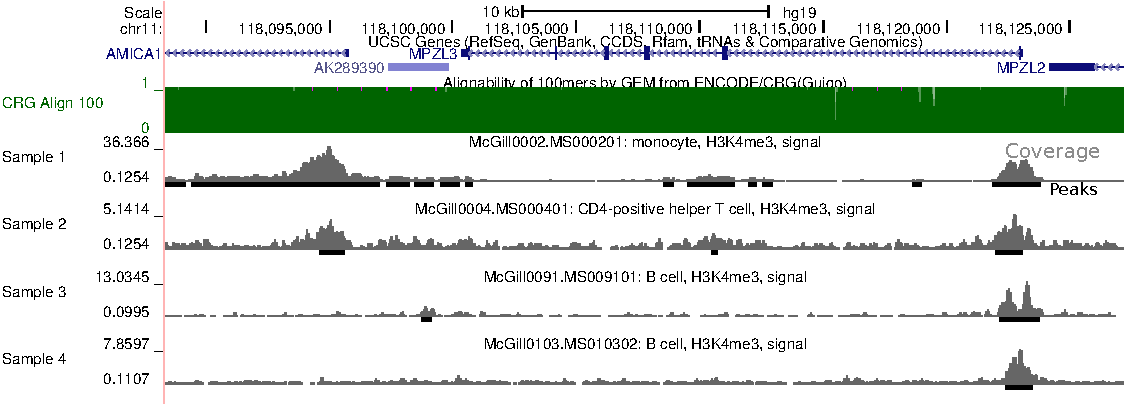
\includegraphics[width=\textwidth]{screenshot-ucsc-edited}

  Grey profiles are normalized aligned read count signals.

  Black bars are ``peaks'' called by MACS2 (Zhang et al, 2008):
  \begin{itemize}
  \item many false positives.
  \item overlapping peaks have different start/end positions.
  \end{itemize}
\end{frame}

\begin{frame}
  \frametitle{Previous work in genomic peak detection}
  \begin{itemize}
  \item Model-based analysis of ChIP-Seq (MACS), Zhang et al, 2008.
  \item SICER, Zang et al, 2009.
  \item HOMER, Heinz et al, 2010.
  \item CCAT, Xu et al, 2010.
  \item RSEG, Song et al, 2011.
  \item Triform, Kornacker et al, 2012.
  \item Histone modifications in cancer (HMCan), Ashoor et al, 2013.
  \item PeakSeg, Hocking, Rigaill, Bourque, ICML 2015.
  \item PeakSegJoint Hocking and Bourque, arXiv:1506.01286.
  \item ... dozens of others.
  \end{itemize}
  Two big questions: how to choose the best...
  \begin{itemize}
  \item ...algorithm? (testing)
  \item ...parameters? (training)
  \end{itemize}
\end{frame}

\begin{frame}[fragile]
  \frametitle{How to choose parameters of unsupervised peak
    detectors?}
\scriptsize
19 parameters for Model-based analysis of ChIP-Seq (MACS), Zhang et al, 2008.
\begin{verbatim}
  [-g GSIZE]
  [-s TSIZE] [--bw BW] [-m MFOLD MFOLD] [--fix-bimodal]
  [--nomodel] [--extsize EXTSIZE | --shiftsize SHIFTSIZE]
  [-q QVALUE | -p PVALUE | -F FOLDENRICHMENT] [--to-large]
  [--down-sample] [--seed SEED] [--nolambda]
  [--slocal SMALLLOCAL] [--llocal LARGELOCAL]
  [--shift-control] [--half-ext] [--broad]
  [--broad-cutoff BROADCUTOFF] [--call-summits]
\end{verbatim}
10 parameters for Histone modifications in cancer (HMCan),
Ashoor et al, 2013.
\begin{verbatim}
minLength 145
medLength 150
maxLength 155
smallBinLength 50
largeBinLength 100000
pvalueThreshold 0.01
mergeDistance 200
iterationThreshold 5
finalThreshold 0
maxIter 20
\end{verbatim}
\end{frame}


\begin{frame}
  \frametitle{Training: select parameter with minimal incorrect labels}
  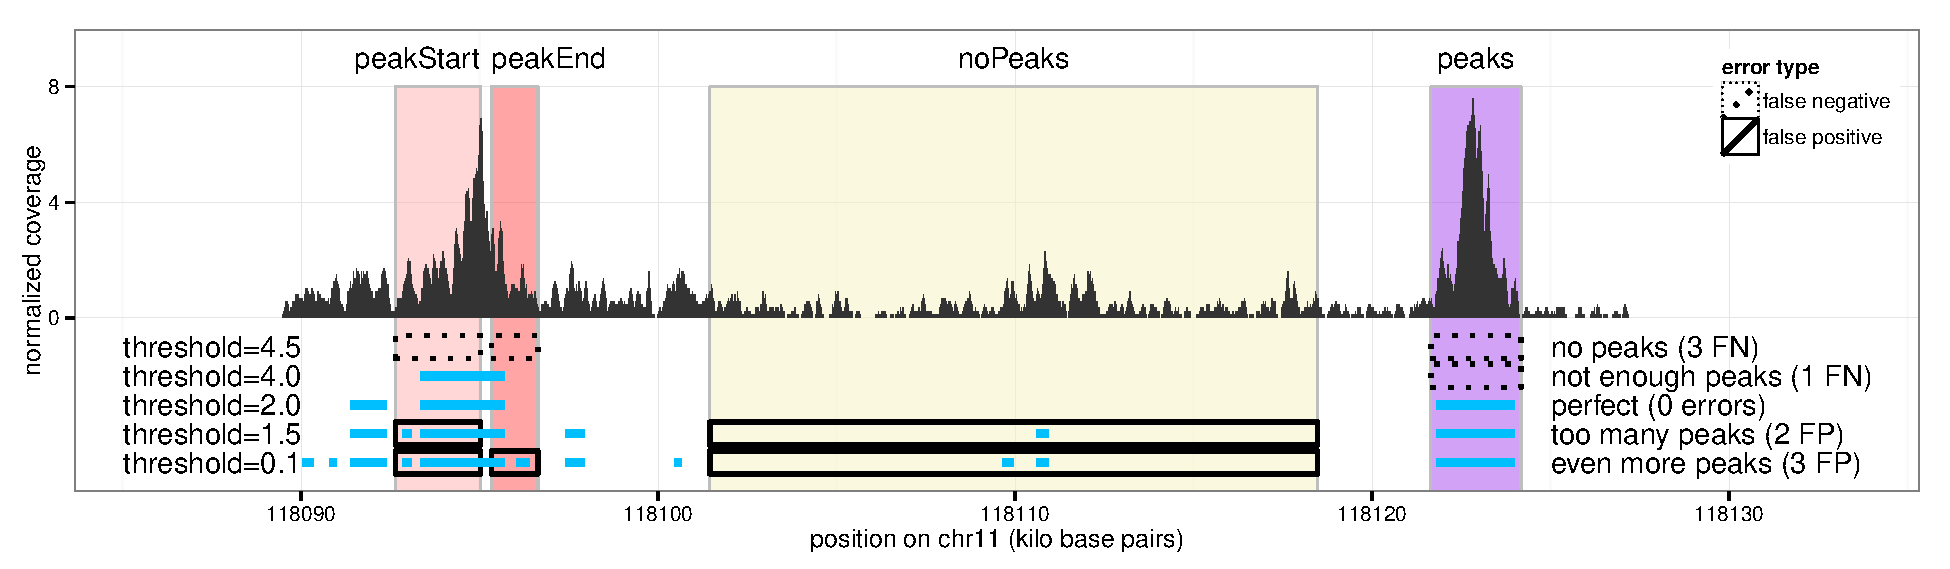
\includegraphics[width=\textwidth]{figure-PeakError.pdf}
  \begin{itemize}
  \item \textbf{peakStart}: exactly one peak start (0=FN, more=FP).
  \item \textbf{peakEnd}: exactly one peak end (0=FN, more=FP).
  \item \textbf{noPeaks}: no overlapping peaks (otherwise FP).
  \item \textbf{peakEnd}: at least one overlapping peak (otherwise FN).
  \end{itemize}
\end{frame}



\begin{frame}
  \frametitle{Training: select parameter with minimal incorrect labels}
  \begin{itemize}
  \item One ChIP-seq sample with $B$ bases $\mathbf z
    \in\ZZ_+^{B}$ of count data.
  \item Set of regions/labels $L$,\\
    e.g. $\{(100, 200, \text{noPeaks}), (500, 650, \text{peakStart})\}$.
  \item \textbf{Training}: use parameters $\lambda$ for a peak caller
    $c_\lambda:\ZZ_+^{B} \rightarrow \{0,1\}^{B}$ such that
  \begin{equation*}
    \label{eq:min_train_err}
    \hat \lambda = 
    \argmin_\lambda
    \sum_{i\in\text{\alert{train}}} E[c_\lambda(\mathbf z_i),  L_i],
  \end{equation*}
  where $E$ is the number of incorrect labels\\(false positives + false
  negatives).
\item \textbf{Not}: use parameters $\lambda$ that recover the ``true'' peaks\\
  (nobody knows, without further experiments).
\item \textbf{Instead}: \alert{use parameters $\lambda$ most
  consistent with the labels in the train set.}
\end{itemize}
\end{frame}

\begin{frame}
  \frametitle{Testing: best algorithm has minimal incorrect labels}
  \begin{itemize}
  \item One ChIP-seq sample with $B$ bases $\mathbf z
    \in\ZZ_+^{B}$ of count data.
  \item Set of regions/labels $L$,\\
    e.g. $\{(100, 200, \text{noPeaks}), (500, 650, \text{peakStart})\}$.
  \item \textbf{Testing}: find a peak caller $c:\ZZ_+^{B} \rightarrow
    \{0,1\}^{B}$ 
  \begin{equation*}
    \label{eq:min_test_err}
    \minimize_c \sum_{i\in\text{\alert{test}}} E[c(\mathbf z_i),  L_i],
  \end{equation*}
  where $E$ is the number of incorrect labels\\(false positives + false
  negatives).
\item \textbf{Not}: find the ``true'' peaks\\
  (nobody knows, without further experiments).
\item \textbf{Goal}: \alert{consistent peak predictions on a held-out
    test set\\ (all the genomic regions and/or samples that you do not
    have time to manually label).}
\end{itemize}
\end{frame}



\begin{frame}
  \frametitle{Accuracy benchmark: 10 manually labeled data sets}
  \url{http://cbio.ensmp.fr/~thocking/chip-seq-chunk-db/}
  \begin{itemize}
  \item We created 12,826 labels in 7 new data sets.
  \item 4 annotators (AM, TDH, PGP, XJ).
  \item 8 cell types.
  \item 37 H3K4me3 samples (sharp peak pattern).
  \item 29 H3K36me3 samples (broad peak pattern).
  \end{itemize}
  \vskip 1cm
  \url{http://tare.medisin.ntnu.no/chipseqbenchmark/}
  \begin{itemize}
  \item 3 data sets from another group's work in 2011.
  \item 3 transcription factors: SRF, NRSF, MAX.
  \item 2 replicates per transcription factor.
  \item Different protocol: label after peak calling.
  \end{itemize}
\end{frame}

\begin{frame}
  \frametitle{Train sets of different sizes, test on same set}
  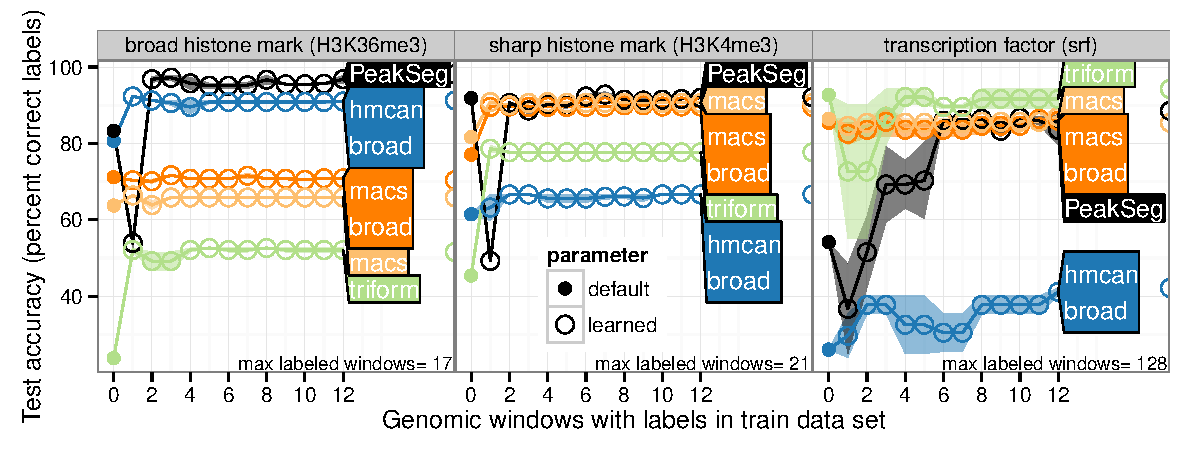
\includegraphics[width=1.1\textwidth]{figure-test-error-decreases-mean.pdf}
\end{frame}

\begin{frame}
  \frametitle{Two annotators provide consistent labels, but different
    precision}
  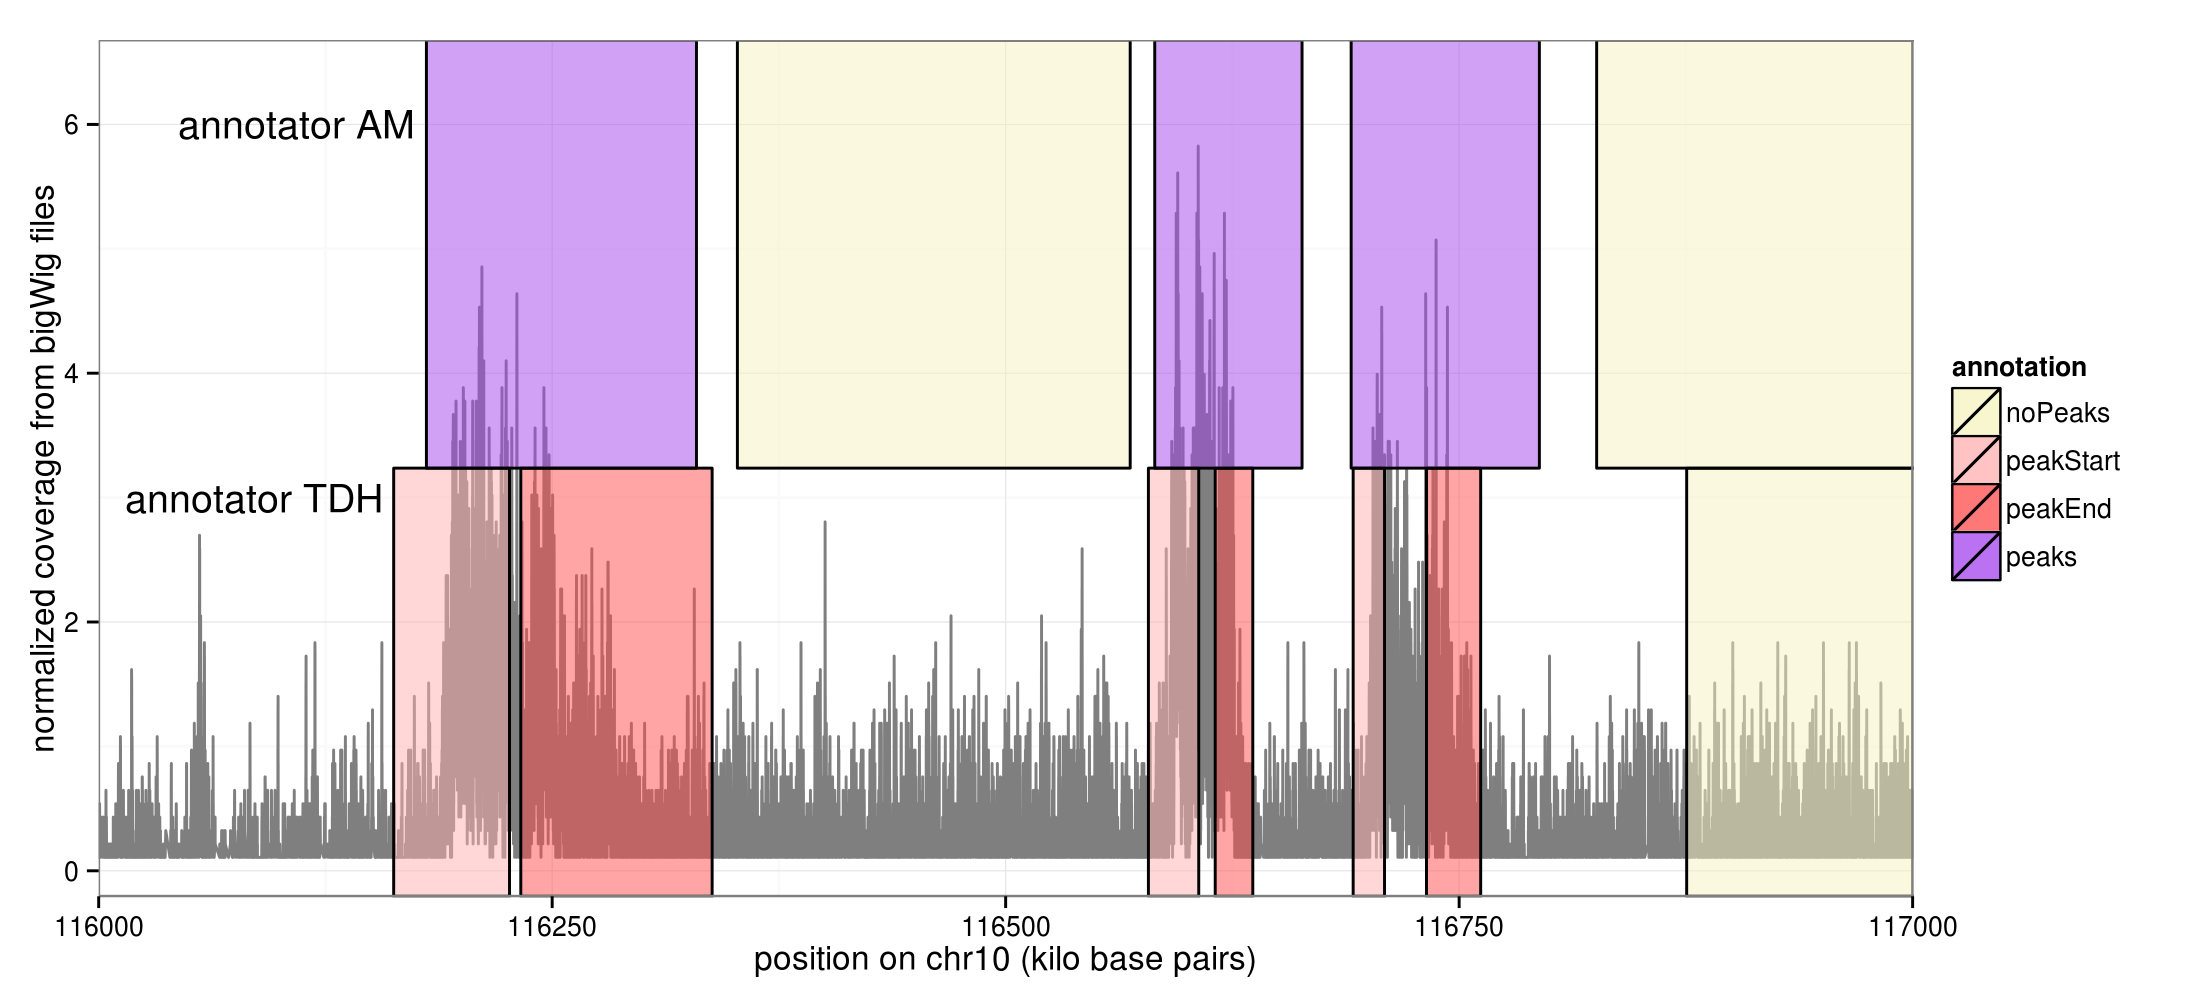
\includegraphics[width=1.1\textwidth]{screenshot-several-annotators}

  \begin{itemize}
  \item TDH peakStart/peakEnd more precise than AM peaks.
  \item AM noPeaks more precise than TDH no label.
  \end{itemize}
\end{frame}

\begin{frame}
  \frametitle{Train on one person, test on another\\
(same histone mark and samples)}
  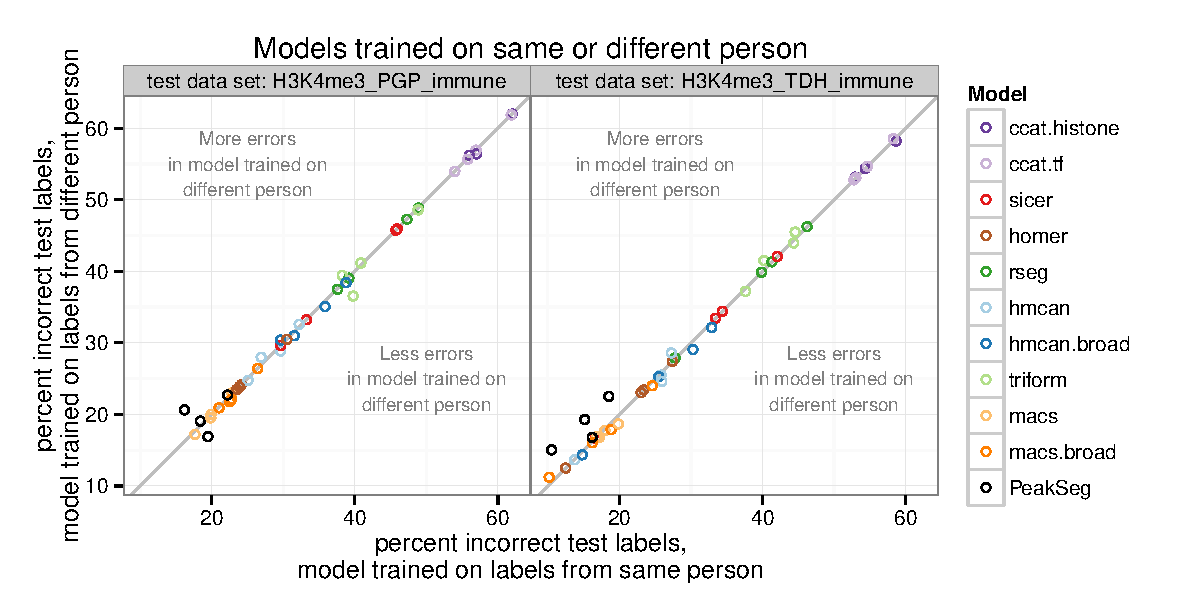
\includegraphics[width=1.1\textwidth]{figure-test-H3K4me3-annotators.pdf}
\end{frame}

\begin{frame}
  \frametitle{Train on some samples, test on others\\
(same histone mark and person)}
  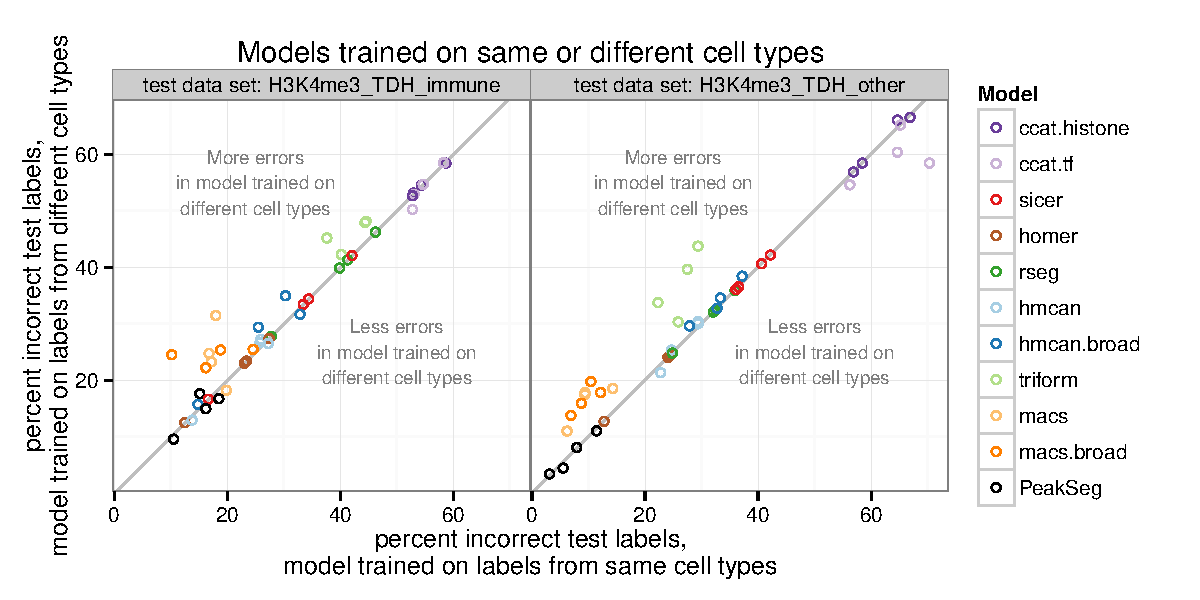
\includegraphics[width=1.1\textwidth]{figure-test-H3K4me3-types.pdf}
\end{frame}

\begin{frame}
  \frametitle{Train on one histone mark, test on another\\
(same person and samples)}
  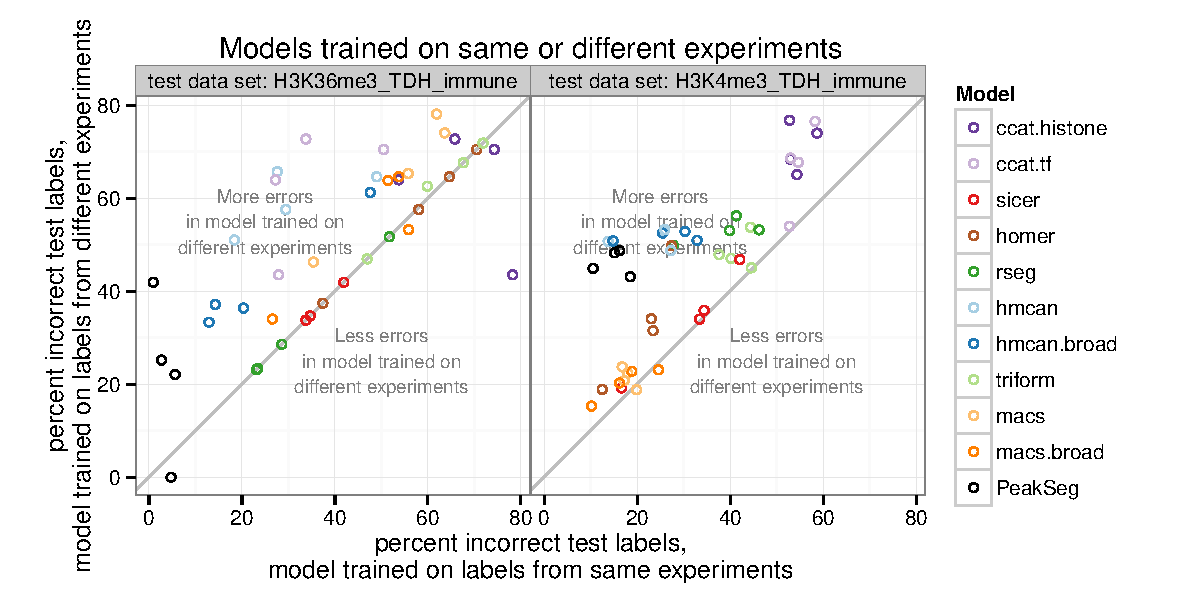
\includegraphics[width=1.1\textwidth]{figure-test-TDH-experiments.pdf}
\end{frame}


\begin{frame}[fragile]
  \frametitle{Unsupervised peak detector input: data + parameters}
\scriptsize
19 parameters for Model-based analysis of ChIP-Seq (MACS), Zhang et al, 2008.
\begin{verbatim}
  [-g GSIZE]
  [-s TSIZE] [--bw BW] [-m MFOLD MFOLD] [--fix-bimodal]
  [--nomodel] [--extsize EXTSIZE | --shiftsize SHIFTSIZE]
  [-q QVALUE | -p PVALUE | -F FOLDENRICHMENT] [--to-large]
  [--down-sample] [--seed SEED] [--nolambda]
  [--slocal SMALLLOCAL] [--llocal LARGELOCAL]
  [--shift-control] [--half-ext] [--broad]
  [--broad-cutoff BROADCUTOFF] [--call-summits]
\end{verbatim}
10 parameters for Histone modifications in cancer (HMCan),
Ashoor et al, 2013.
\begin{verbatim}
minLength 145
medLength 150
maxLength 155
smallBinLength 50
largeBinLength 100000
pvalueThreshold 0.01
mergeDistance 200
iterationThreshold 5
finalThreshold 0
maxIter 20
\end{verbatim}
\end{frame}

\begin{frame}
  \frametitle{Training: select parameter with minimal incorrect labels}
  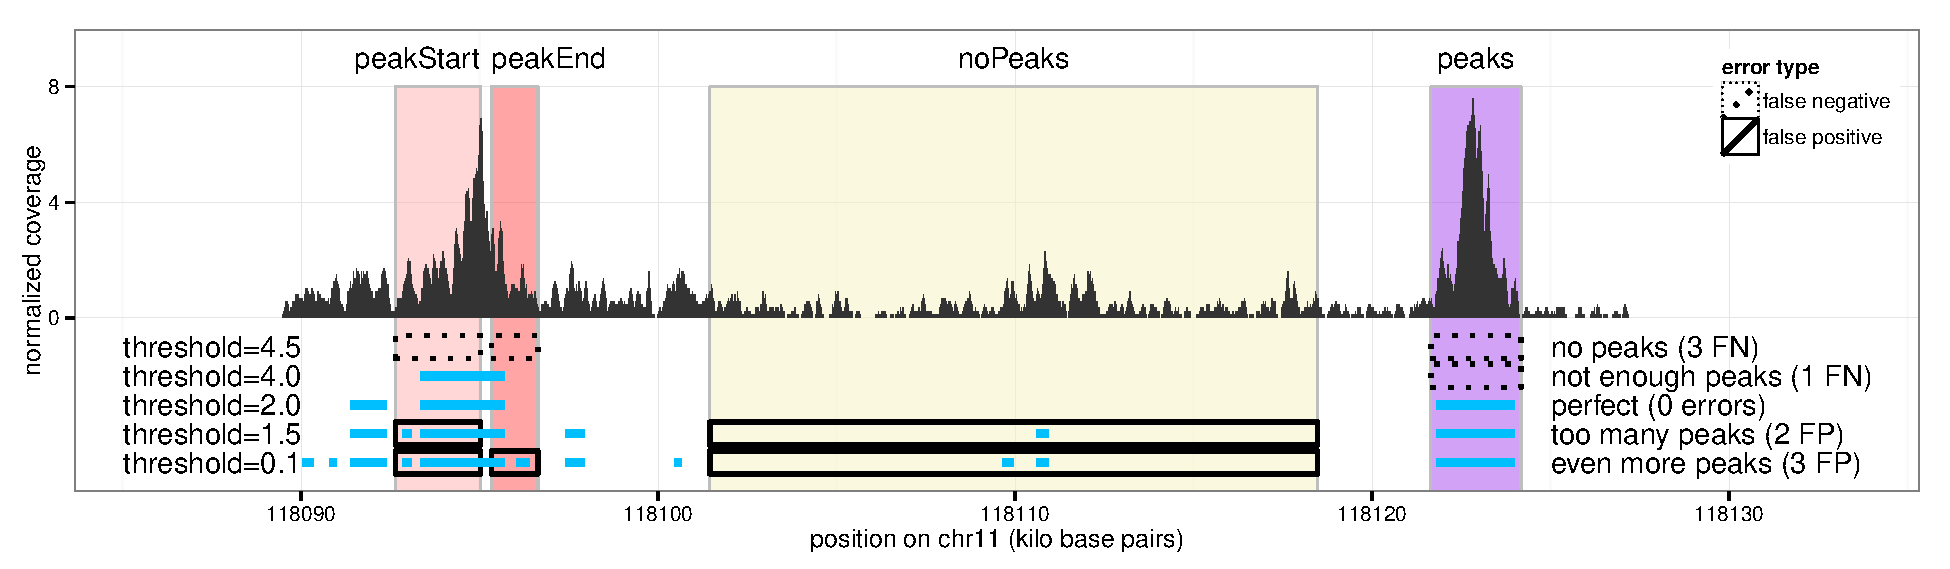
\includegraphics[width=\textwidth]{figure-PeakError.pdf}
  \begin{itemize}
  \item \textbf{peakStart}: exactly one peak start (0=FN, more=FP).
  \item \textbf{peakEnd}: exactly one peak end (0=FN, more=FP).
  \item \textbf{noPeaks}: no overlapping peaks (otherwise FP).
  \item \textbf{peakEnd}: at least one overlapping peak (otherwise FN).
  \end{itemize}
\end{frame}

\begin{frame}
  \frametitle{New labeling step in ChIP-seq pipelines}
  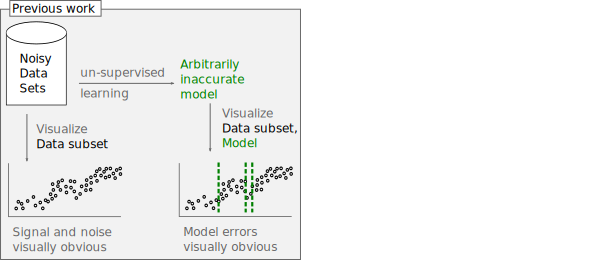
\includegraphics[width=0.9\textwidth]{GenomicLearner-unsupervised.pdf}
\end{frame}

\begin{frame}
  \frametitle{New labeling step in ChIP-seq pipelines}
  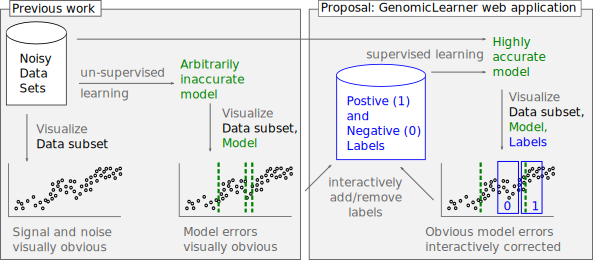
\includegraphics[width=0.9\textwidth]{GenomicLearner-both.pdf}
\end{frame}


\begin{frame}
  \frametitle{Conclusions and future work}
  \begin{itemize}
  \item \textbf{New method}: supervised peak detection.
  \item \textbf{Benefits}: more user-friendly, accurate.
  \item \textbf{Fast learning}: only 5-10 labeled genomic windows are
    necessary for state-of-the-art accuracy.
  \item \textbf{Generalization} between labels from different people,
    and samples of different cell types (not different experiments).
\end{itemize}
 \textbf{TODO}: web app for interactive ChIP-seq data analysis, featuring
\begin{itemize}
  \item Simultaneous visualization of coverage, labels, and peak predictions.
  \item Click to add new labels or delete existing labels.
  \item After changing the labels, update the machine learning model
    and the displayed peak predictions.
  \end{itemize}
\end{frame}

\begin{frame}
  \frametitle{Thanks for your attention!}
  Write me at \alert{\texttt{toby.hocking@mail.mcgill.ca}} to collaborate!

  \vskip 1cm

  R packages:\\
  \url{https://github.com/tdhock/PeakError}\\
  \url{https://github.com/tdhock/PeakSegJoint}

  \vskip 1cm

  Source code for slides, figures, paper online!\\
  \small
  \url{https://bitbucket.org/mugqic/chip-seq-paper}
  \vskip 1cm

  Supplementary slides appear after this one.

\end{frame}

\begin{frame}
  \frametitle{Test error in three different experiments}
  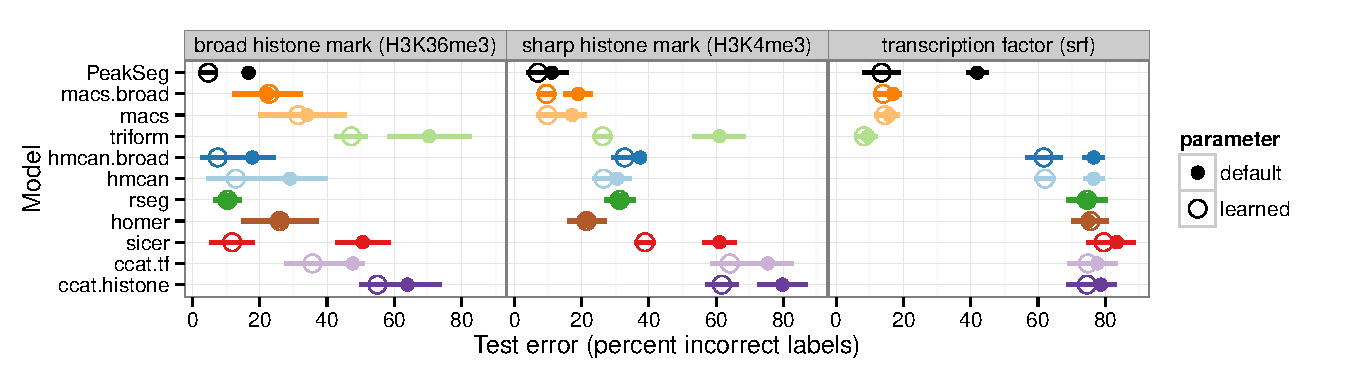
\includegraphics[width=1.1\textwidth]{figure-test-error-dots-mean.pdf}
\end{frame}

\end{document}
